\section{Method}\label{sec:method}
This section describes the steps of our method on an abstract level.
\todo{ref pipelinefigure} visualizes these steps as a flowchart.
Each step of the method is described later in more detail. 

We start with a dataset, in our case consisting of news articles from the media group Nordjyske. 
Their primary focus is to maintain a variety of local newspapers within the North Jutland region of Denmark. 
The data ranges from 2017, where a total of $\sim$~63.000 articles have been extracted from their database.

\subsection*{Step 1: Preprocessing Phase}
This phase applies different \gls{NLP} methods, such as stemming and removing stop words, to simplify the data set and remove redundant information.
Details of this phase are given in \autoref{sec:prepro}.
After finishing this phase, we are left with $\sim$32.000 documents, which will be used in future steps.

\subsection*{Step 2: LDA}
We train a \acrfull{lda} model on the dataset to generate topics based on the content of articles within the dataset. 
We describe the investigation and selection of hyper parameters in \autoref{subsec:hyperparameters}. 
After the model has been trained, we have a document-topic distribution matrix $\theta$ and a topic-word distribution matrix $\beta$.

\subsection*{Step 3: Query Preprocessing}
A search query, consisting of words, is stemmed and turned into a list of words.
For each word, we generate a topic distribution based on topic-word distribution $\beta$ if the model knows the words within the query.
Otherwise, we let the model predict which topics the unknown words belong to.
We use the final distribution, as a personalization vector for our PageRank combination models.
\todo[inline]{Check that the description of how the personalization vector is made, is correct}
The output of this step is a list of search queries.


\subsection*{Step 4: Evaluation of models}
In this phase, we evaluate different combinations of models using the evaluation metrics described in \todo{ref evaluation metric section}.
The evaluation is done by testing the search queries against the different models. 
The combinations and results can be seen in section \todo{ref combination section } and \todo{ref result section }, respectively.


\tikzstyle{process} = [rectangle, rounded corners, minimum width=2cm, minimum height=1cm,text centered, draw=black, fill=gray!50]

\begin{figure}[h]
    \centering
    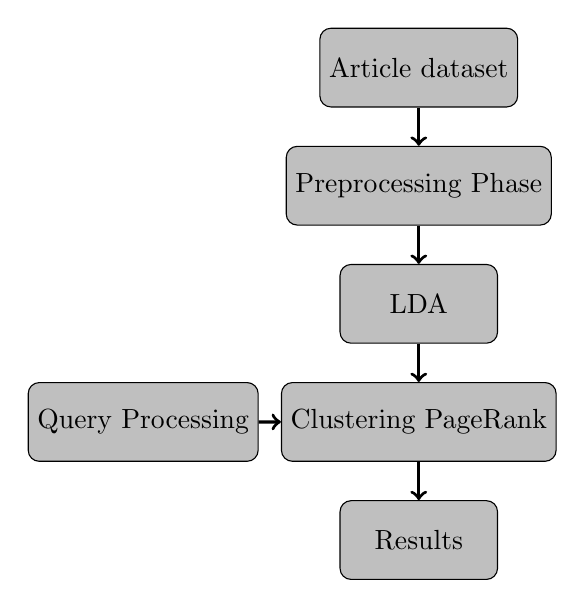
\begin{tikzpicture}[node distance=1.5cm]
    %\draw[step=1cm,gray,very thin] (-8,-8) grid (8,8);
	\node (Dataset) [process] {Article dataset};
	\node (Cleaning)[process, below of=Dataset] {Preprocessing Phase};
	\node (Training) [process, below of=Cleaning] {LDA};
	\node (Cluster PR) [process, below of=Training] {Clustering PageRank};
	\node (Query) at (-3.5, -4.5) [process] {Query Processing};
	\node (Result) [process, below of=Cluster PR] {Results};
	\draw [->, very thick] (Dataset) edge (Cleaning); 
	\draw [->, very thick] (Cleaning) edge (Training);
	\draw [->, very thick] (Training) edge (Cluster PR);
	\draw [->, very thick] (Cluster PR) edge (Result);
	\draw [->, very thick] (Query) edge (Cluster PR);
\end{tikzpicture}
	\caption{Pipeline}
    \label{fig:pipeline}
\end{figure}
